\begin{tabular}{ | p{2cm} | p{14cm} | } 
	\hline
	Név: &Szeifert Anita aosj4d\\ 
	\hline
	Szak: & Anyagmérnök \\ 
	\hline
	Félév: & 2019/2020 II. (tavaszi) félév \\ 
\hline
\end{tabular}
\vspace{5mm}
\\HS10 feladat:\\
Stacioner viszonyok esetében egy samott gömbnél az alábbi adatokkal határozza meg a $d_{koz}$ átmérőjű izoterm gömbfelület hőmérsékletét $(T_2)$.
\section*{ {Adatok:}}

$
\lambda=\SI[per-mode=fraction]{1,395}{\watt\per\meter\per\kelvin}D_1 =\SI{0,6}{meter} D_2 =\SI{1}{\meter} T_2=\SI{1023,15}{\kelvin}=\SI{750}{\degreeCelsius}
$
\vspace{1mm}
\section {Feladat megoldás}

A Fourier -egyenlet integrálásával kapott hőmennyiség egyenlete

\begin{equation}
	\dot{Q}=\dfrac{4\pi \lambda(T_1-T_2)}{\dfrac{1}{r_1}-\dfrac{1}{r_2}}
\end{equation}

\vspace{10mm}
Behelyettesítve az egyenletbe:
\begin{equation}
\SI{4186,8}{\watt}=\dfrac{4\pi\SI[per-mode=fraction]{1,395}{\watt\per\meter\per\kelvin}}
{\dfrac{1}{\SI{0.3}{\meter}}-\dfrac{1}{\SI{0,5}{\meter}}}
\hspace{1mm} (\SI{1023,15}{\kelvin}-T_2)
\end{equation}

%\vspace{10mm}
Rendezések után azt kapjuk, hogy 
\begin{equation*}
    T_2=\SI{704,71}{\kelvin}=\SI{431,56}{\degreeCelsius}
\end{equation*}
   

\begin{figure}[h]
\centering
    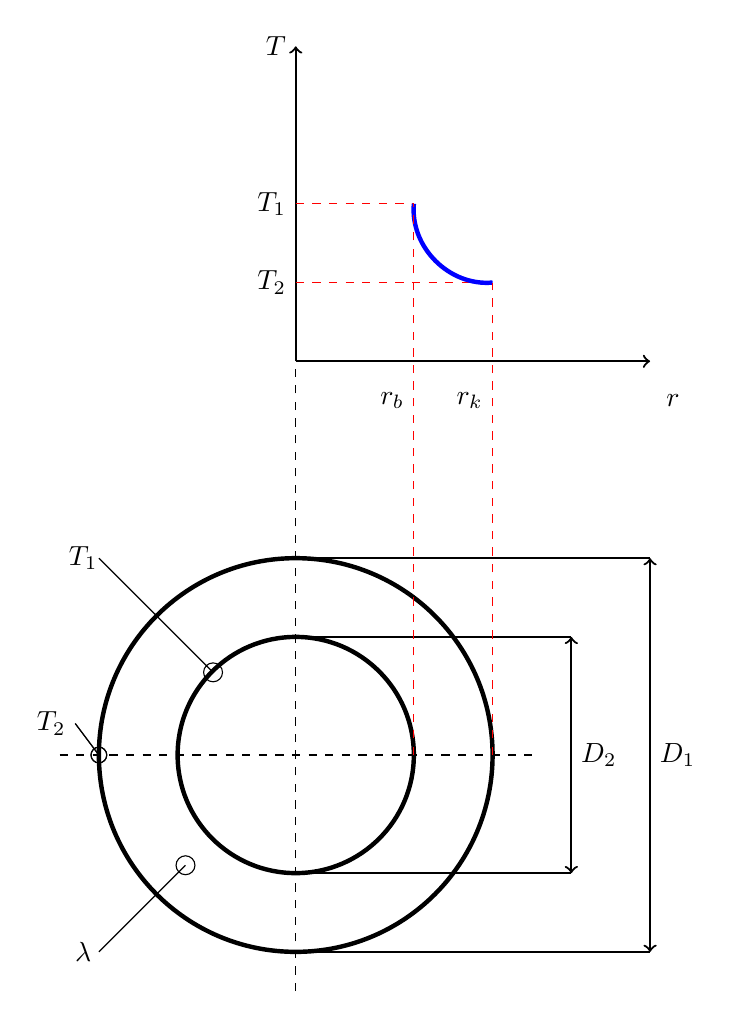
\begin{tikzpicture}
        %\draw[] (-6, -6) rectangle (6, 6); rajz keret
        \draw[color =black, ultra thick] (0,0) circle (25mm); %belső fal
        \draw[color =black,ultra thick] (0,0) circle (15mm ) ;%külső fal
        %r tengely
        \draw[thick,->] (0,50mm) -- (45mm,50mm);% méretnyíl
        %D1 vetítő vonala
        \draw[thick] (0,25mm) -- (45mm,25mm);
        \draw[thick] (0,-25mm) -- (45mm,-25mm);
        \draw (45mm,0)  node[right] {$\diameter D_1  $};
        \draw [thick,<->] (45mm,25mm) -- (45mm,-25mm);
        
        %T tengely
        \draw[thick,->] (0mm,50mm) -- (0mm,90mm);
        %r_k,b
        \draw (0,45mm)  (25mm,45mm)  node[left] {$ r_k  $};
        \draw (0,45mm)  (15mm,45mm)  node[left] {$ r_b  $};
        \draw (0,45mm)  (50mm,45mm)  node[left] {$ r $};
        \draw (0,45mm)  (0,90mm)  node[left] {$ T $};
        %T1,2 pont a t tengelyen
        \draw (0,45mm)  (0,70mm)  node[left] {$ T_1 $};
         \draw (0,45mm)  (0,60mm)  node[left] {$ T_2$};
        % T tengely piros vonalai
        \draw[thin,dashed,red](0,70mm) --(15mm,70mm);
        \draw[thin,dashed,red](0,60mm) --(25mm,60mm);
        %D2 méret vonalai
        \draw[thick] (0,15mm) -- (35mm,15mm);% méretnyíl
        \draw[thick] (0,-15mm) -- (35mm,-15mm);% méretnyíl
        \draw[thick,<->] (35mm,15mm) -- (35mm,-15mm);% méretnyíl
        \draw (35mm,0)  node[right] {$\diameter D_2  $};
        \draw[color=blue, ultra thick] (15mm,70mm) to [bend right=50] (25mm,60mm);
        ;
        %\draw[thick,<->] (-3.5,4.5) -- (3.5,4.5); %felső méretnyíl
        %\draw (0,4.5)  node[above] {$ D_2  $};
        %Tengely keresz
        \draw[thin,dashed,black](-30mm,0) --(30mm,0);
        %\draw[thin](-30mm,0) -(30mm,0);
        \draw[thin,dashed,red](15mm,0) --(15mm,70mm);
        \draw[thin,dashed,red](25mm,0) --(25mm,60mm);%nagysugár felszaggatott
        \draw [thin] (-25mm,0) circle (0.1) (-25mm,0) -- (-28mm,4mm); 
        \draw[thin,dashed,black](0,-30mm) --(0,50mm);

%T1
\draw [thin] (-10.5mm,10.5mm) circle (0.12) (-10.5mm,10.5mm) -- (-25mm,25mm)  ;
\draw [thick]( -27mm,25mm)  node[] {$T_1$};
 %lambda 
 \draw [thin] (-14mm,-14mm) circle (0.12) (-14mm,-14mm) -- (-25mm,-25mm)  ;
 \draw [thick]( -27mm,-25mm)  node[] {$\lambda$};
 %T2
\draw [thin] (-25mm,0) circle (0.1) (-25mm,0) -- (-28mm,4mm)  ;
\draw (-28mm,4mm)  node[left] {$T_2$};

        \end{tikzpicture}
    \caption{Samott gömbfal hőmérséklet-hely függvénye}
    \end{figure}
%\begin{figure}
%	\centering
%	\includegraphics[width=1\linewidth]{h5omersekletfuggvenyHS10.eps}
%	\caption{}
%	\label{fig:waveforms}
%\end{figure}

\end{document}
